\question A thin, semi-circular ring of radius $R$ carries a total charge $+Q$. A distance $R$ to the left of the center of the ring is a thin negatively charged rod carrying charge $-Q$. The length of the rod is the same as the diameter of the ring: $2R$. Using the coordinate directions defined in the figure, what is the electric field vector at point $A$, which is at the center of the semi-ring and lies along the middle axis of the rod? Express your answer in terms of the variables defined in the problem: $Q$ and $R$, as well as the constant $\epsilon_0$ or $k$. You do not need to evaluate any integrals that arise (you may express your answer in the form of one or more integrals, but make sure to specify the bounds of integration).
\begin{center}
	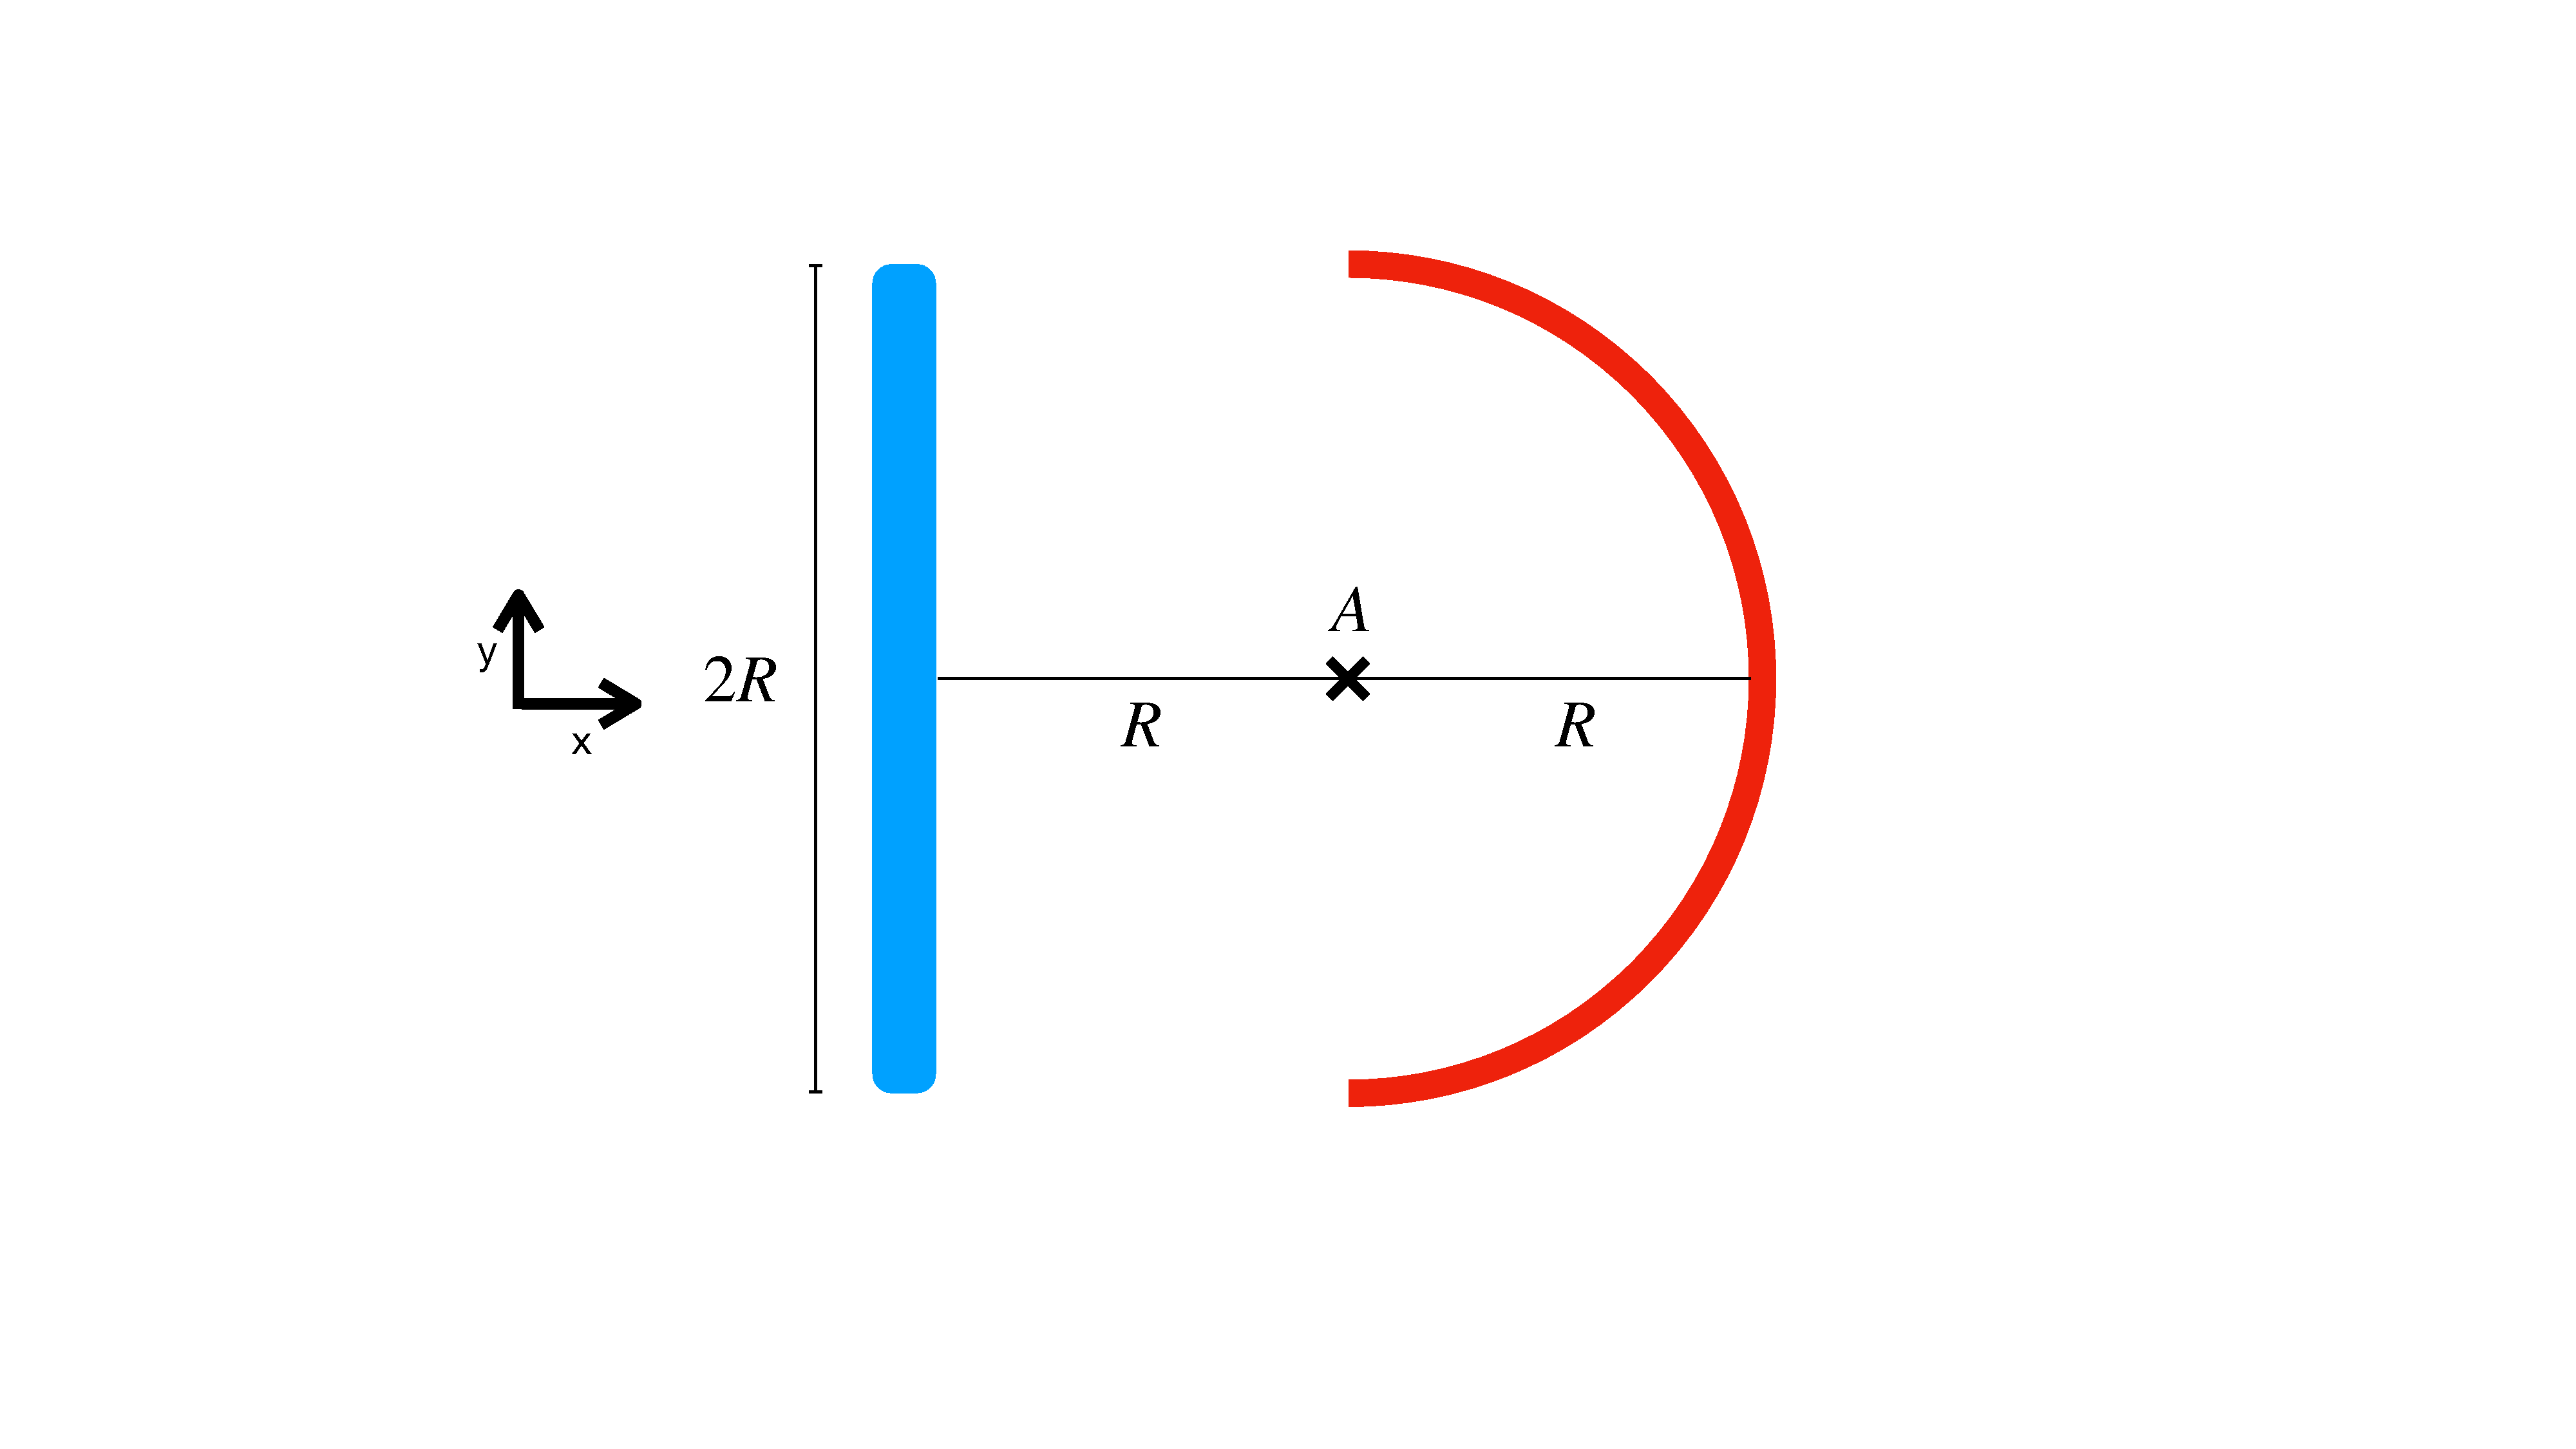
\includegraphics[width=.5\textwidth]{p6diag1}
\end{center}